	\section{Introduction}
	parlare dell'iot in generale ...
	
	\subsection{Structure of an IoT application}
	Most of the time an IoT system is a large scale application that put in place different protocol, different hardware
	and different software.\newline
	From the protocols point of view there are lots of choices, just to list someone: HTTP, MQTT, WebSocket and CoAP;
	each one has advantages and disadvantages, so it is crucial to choose the one that fits well your business logic; also take in mind
	that some protocols like MQTT or CoAP are used in sensors-server communication, while HTTP and WebSocket
	are used for client-server communications.\newline
	While dealing with IoT we can encounter lots of different hardware: from the constrained device with low computational power to
	high performance cluster machine, basically the dirty work is taken over by lots of low power devices which communicate to the server,
	that will elaborate this data or forward it to the cloud in order to elaborate them in a fastest way.\newline
	On the software front we can work with a variety of programming languages: from low level assembly to high level languages like C\# or JavaScript.\newline
	The development of an IoT system also requires a deep knowledge of the different parts of the application, so the development team
	should be formed by people with different skill and specialization. <-- mi sembra sensato, ma vorrei una conferma\newline
	This little overview should help you to understand how difficult could be to design and develop an IoT application, figure \ref{fig:intro0} illustrates 
	a schematic view of the architecture of an IoT application.\newline
	
	\begin{figure}
		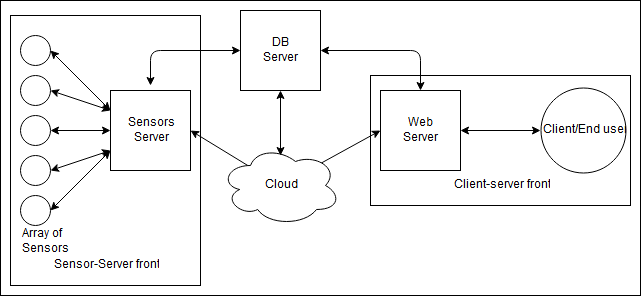
\includegraphics[width=\linewidth]{intro-000.png}
		\caption{Possible architecture of an IoT application.}
		\label{fig:intro0}
	\end{figure}
	
	\subsection{Argument of the thesis}
	
	In this thesis I will analyze two IoT protocol: CoAP and WebSocket.\newline
	These two protocols were chosen because they allow me to show how communication occurs on two different front:
	the sensor-server: where the server collects incoming data from the sensors, then the server proceed with some elaborations, it depends on the application targets but the most common elaborations are: monitoring, machine learning and statistics; and the client-server front, where the client requests data from the server in order to show them to
	the final user.\newline

	CoAP is a protocol that works on the sensor-server part of the application, while WebSocket focus
	on the client/server side, WebSocket is more flexible compared to CoAP, it can be used even for
	jobs that where not taken into account during its design phase, while CoAP is a very specialized
	protocol that fits well only in certain constrained scenarios.\newline
	WebSocket could be used on the sensor-server side but, as we will analyze in details during the next chapter,
	we are going to deal with constrained devices that may lack the proper resources to implement the protocol in the correct way.\newline
	
	After analyzing the two protocols, I will focus on their vulnerabilities and possible attacks to show
	how important is to use them in a safe way in order to achieve security in IoT applications.\newline
	It is important to highlight that both communications: sensors-server and client-server must be secure in order to guarantee
	the security of the whole application, that is because if the sensors-server is secure but the client-server is not, then an
	attacker could compromise the entire application while acting only on one front; of course this is true even for the other way around.\newline
	
	For the client-server front, I will list the best practice to write a secure application, this section of the thesis
	is a mix of previous knowledges learned during the security course attended in the first year of the MsC and new one
	acquired during the internship at Abo Data.\newline
	
	At the end I will describe my personal experience in the company; I worked on two real IoT applications and we will
	discuss them in order to have an in-depth overview of IoT applications.\newline
	Then I will describe the security flaws detected and how it was possible to fix them and evaluate how difficult it was.\newline
	To conclude I will analyze how security influences the development of an application and the reasons why sometimes it is neglected,
	in the end I will discuss how security should be an important part during the design and development phase of an application
	and not a final add-on for the system.\newline
	
	
	